Die Untersuchung der zur Zeit eingesetzten Sofware beschränkt sich auf jene,
die einen direkten Einfluss auf den aktuellen Projektablauf bei allink haben.
Es wird keine Software aufgelistet, die zur Erbringung der eigentlichen 
Dienstleistungen im Unternehmen eingesetzt wird.

\begin{center}
    \begin{longtable}{lllp{6cm}}
        \toprule \textbf{Bezeichnung} & \textbf{Hersteller} & \textbf{Kategorie} & \textbf{Verwendungszweck} \\
        \midrule MacOS X & Apple & Betriebssystem & 
            \begin{minipage}[t]{6cm}
                \begin{compactitem}
                    \item Über den ganzen Projektablauf
                \end{compactitem}
            \end{minipage}
            \\\\
        \midrule Microsoft Windows & Microsof & Betriebssystem & 
            \begin{minipage}[t]{6cm}
                \begin{compactitem}
                    \item Tests während der Entwicklung
                    \item Präsentation in der Abnahme
                \end{compactitem}
            \end{minipage}
            \\\\
        \midrule MacOS X Server & Apple & Betriebssystem &
            \begin{minipage}[t]{6cm}
                \begin{compactitem}
                    \item Zentrale Dateiablage
                    \item Server des Stundenwidgets
                    \item Internes Wiki der Informatik
                \end{compactitem}
            \end{minipage}
            \\\\
        \midrule Apple iWork & Apple & Office Suite &
            \begin{minipage}[t]{6cm}
                \begin{compactitem}
                    \item Kalkulation von Offerten
                    \item Erstellung von Offerten
                    \item Erstellung von Rechnungen und Briefschaften
                \end{compactitem}
            \end{minipage}
            \\\\
        \midrule Microsoft Office & Microsoft & Office Suite &
            \begin{minipage}[t]{6cm}
                \begin{compactitem}
                    \item Informationsaustausch mit Kunden
                \end{compactitem}
            \end{minipage}
            \\\\
        \midrule Apple Mail & Apple & E-Mail Software &
            \begin{minipage}[t]{6cm}
                \begin{compactitem}
                    \item Korrespondenz mit Kunden
                    \item Interne Kommunikation
                \end{compactitem}
            \end{minipage}
            \\\\
        \midrule Stundenwidget & allink & Dashboardwidget &
            \begin{minipage}[t]{6cm}
                \begin{compactitem}
                    \item Stundenrapportierung
                \end{compactitem}
            \end{minipage}
            \\\\
        \bottomrule
        \caption{Verwendete Software bei allink}
        \label{tab:verwendete_software}
    \end{longtable}
\end{center}

\subsubsection{MacOS X}
Als Hauptbetriebssystem verwendet allink MacOS X\footnote{Betriebssystem von Apple, \url{http://www.apple.com/macosx/}}.
Es läuft auf allen Arbeitsstationen der Mitarbeiter und Partner. Dies beruht
auf diversen Gründen. Grafiker arbeiten überwiegend mit MacOS X, da sich Apple
früh mit Adobe zusammenschloss um Werkzeuge für Grafiker zur Verfügung zu stellen.
Seit mehreren Jahren ist MacOS X auch für Entwickler wieder interessant. Die 
Mitarbeiter sind gemäss dem Auftraggeber sehr zufrieden damit und die Geschäftsleitung 
möchte dies zu diesem Zeitpunkt nicht in Frage stellen.

\subsubsection{Microsoft Windows}
Zusätzlich haben einige der Entwickler noch Microsoft Windows\footnote{Betriebssystem von Microsoft, \url{http://www.microsoft.com/windows/}}
über eine Virtualisierungslösung installiert. Dies wird zu überwiegend Testzwecken 
benötigt. Es existiert zu diesem Zeitpunkt aber kein Rechner, der ausschliesslich
mit Microsoft Windows arbeitet.

\subsubsection{MacOS X Server}
Auf dem Server der allink liegt das zentrale Dateiablagesystem. Die Zugriffsrechte können
auf dem Server für jede Freigabe definiert werden. So haben zum Beispiel
die Mitarbeiter keinen Zugriff auf den Administrationsordner der Geschäftsleitung.
Über diesen Server laufen auch die einzelnen Firmenkalender der Partner. Sie
können so gemeinsam Termine buchen und haben stets Einblick in die anderen
Kalender. Auch hier ist sich die Geschäftsleitung einig, zur Zeit keine 
Veränderung vorzunehmen.

\subsubsection{Apple iWork}
Für interne Zwecke setzt allink zur Zeit auf die Apple eigene Office Suite iWork\footnote{Office Suite von Apple, \url{http://www.apple.com/de/iwork/}}.
Pages wird überwiegend zur Erstellung von Offerten und Rechnungen verwendet. Mit Numbers
werden Tabellenkalkulationen wie die Liquiditätsplanung oder Lohnblätter erstellt.
Da dies aber von der Geschäftsleitung nie klar kommuniziert wurde, existieren
auch einige Excel Files, das Pendant der Microsoft Office Suite.

\subsubsection{Microsoft Office}
Da viele Kunden mit Microsoft Produkten arbeiten benötigt auch allink die
Office Suite\footnote{Microsoft Office für Mac, \url{http://www.microsoft.com/germany/mac}}, 
um Dateien mit Kunden ohne Interoperabilitätsprobleme austauschen zu können. 
Nicht jede Arbeitsstation verfügt zur Zeit über eine Installation. Da diese
Suite aber im Vergleich mit Apples iWork einiges teurer in den Anschaffung ist,
möchte die Geschäftsleitung diese über kurz oder lang nur noch auf einzelnen
Arbeitsstationen installieren.

\subsubsection{Apple Mail}
Apple Mail ist in das Betriebssytem von MacOS X integriert und wird gratis
mitgeliefert. Es verfügt über alle nötigen Funktionen, die eine E-Mail-Client-Software
heutzutage erfüllen muss. Auch diese möchte die Geschäftsleitung zur Zeit nicht
in Frage stellen.

\subsubsection{Stundenwidget}
Das Stundenwidget ist eine Eigenentwicklung von allink und läuft
im Dashboard\footnote{Widget Lösung von Apple, \url{http://www.apple.com/downloads/dashboard/}}
des Betriebssystems. Es ermöglicht Stunden auf ein Projekt zu buchen.
% 
% \begin{figure}[htbp]
% \begin{center}
% 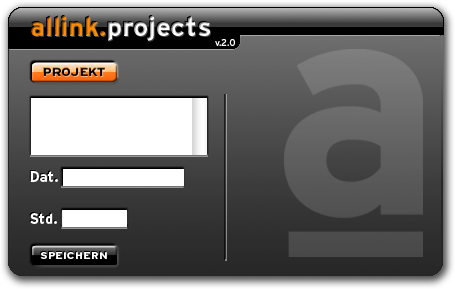
\includegraphics[width=0.3\textwidth,angle=0]{./bilder/analyse/ist_widget.png}
% \caption{Stundenwidget von allink}
% \label{pic:ist_widget}
% \end{center}
% \end{figure}

Die Daten werden auf dem eigenen Server gespeichert und pro Projekt abgelegt. Dieses Widget ist auf allen
Arbeitsstationen installiert und wird von den Mitarbeitern gelegentlich verwendet
um ihre Stunden auf ein Projekt zu rapportieren.
